\documentclass[11pt,fleqn, openany]{book} % Default font size and left-justified equations

%%%%%%%%%%%%%%%%%%%%%%%%%%%%%%%%%%%%%%%%%
% The Legrand Orange Book
% Structural Definitions File
% Version 2.1 (26/09/2018)
%
% Original author:
% Mathias Legrand (legrand.mathias@gmail.com) with modifications by:
% Vel (vel@latextemplates.com)
% 
% This file was downloaded from:
% http://www.LaTeXTemplates.com
%
% License:
% CC BY-NC-SA 3.0 (http://creativecommons.org/licenses/by-nc-sa/3.0/)
%
%%%%%%%%%%%%%%%%%%%%%%%%%%%%%%%%%%%%%%%%%

%----------------------------------------------------------------------------------------
%	VARIOUS REQUIRED PACKAGES AND CONFIGURATIONS
%----------------------------------------------------------------------------------------

\usepackage[table]{xcolor}

\usepackage{graphicx}
\usepackage{tabularx} % Required for including pictures
\usepackage{pgf,tikz,tkz-tab,eurosym,yhmath, stmaryrd}
\usepackage{pgfplots}
\usepackage{mathrsfs}
\usetikzlibrary{patterns}
\usetikzlibrary{trees}
\graphicspath{{../../Pictures/}}
\usepackage{multicol} 


\usepackage[english]{babel} % English language/hyphenation
\usepackage{icomma}
\usepackage{enumitem} % Customize lists
\setlist{nolistsep, nosep, nolistsep} % Reduce spacing between bullet points and numbered lists

\usepackage{booktabs} % Required for nicer horizontal rules in tables

 % Required for specifying colors by name


\definecolor{ocre}{RGB}{243,102,25} % Define the orange color used for highlighting throughout the book

\usepackage{listings}

\definecolor{codegreen}{rgb}{0,0.6,0}
\definecolor{codegray}{rgb}{0.5,0.5,0.5}
\definecolor{codepurple}{rgb}{0.58,0,0.82}
\definecolor{backcolour}{rgb}{0.95,0.95,0.92}

\lstdefinestyle{mystyle}{
    backgroundcolor=\color{backcolour},   
    commentstyle=\color{codegreen},
    keywordstyle=\color{magenta},
    numberstyle=\tiny\color{codegray},
    stringstyle=\color{codepurple},
    basicstyle=\ttfamily\footnotesize,
    breakatwhitespace=false,         
    breaklines=true,                 
    captionpos=b,                    
    keepspaces=true,                 
    numbers=left,                    
    numbersep=5pt,                  
    showspaces=false,                
    showstringspaces=false,
    showtabs=false,                  
    tabsize=2
}

\lstset{style=mystyle}

%----------------------------------------------------------------------------------------
% Paramétrage XSIM
%----------------------------------------------------------------------------------------

\usepackage[no-files]{xsim}


\DeclareExerciseEnvironmentTemplate{myex}{%
    \textbf{%
      \hypertarget{ex:\ExerciseID}{\sffamily{\ensuremath{\blacktriangleright}} Exercice \GetExerciseProperty{counter} \GetExerciseProperty{subtitle} --}
      \hyperlink{sol:\ExerciseID}{Voir le corrigé}%
    }\par
}{\par\smallskip}

\DeclareExerciseEnvironmentTemplate{mysol}{%
    \textbf{%
      \hypertarget{sol:\ExerciseID}{\sffamily{\ensuremath{\blacktriangleright}} Correction \GetExerciseProperty{counter} --}
      \hyperlink{ex:\ExerciseID}{Voir l'énoncé}%
    }\par
}{\par\medskip}

\xsimsetup{
  exercise/template = myex ,
  solution/template = mysol 
}

%Collection exercices

\DeclareExerciseTagging{topic}

\xsimsetup{collect}

%----------------------------------------------------------------------------------------
% SYMBOLES
%----------------------------------------------------------------------------------------

\newcommand\imCMsym[4][\mathord]{%
  \DeclareFontFamily{U} {#2}{}
  \DeclareFontShape{U}{#2}{m}{n}{
    <-6> #25
    <6-7> #26
    <7-8> #27
    <8-9> #28
    <9-10> #29
    <10-12> #210
    <12-> #212}{}
  \DeclareSymbolFont{CM#2} {U} {#2}{m}{n}
  \DeclareMathSymbol{#4}{#1}{CM#2}{#3}
}
\newcommand\alsoimCMsym[4][\mathord]{\DeclareMathSymbol{#4}{#1}{CM#2}{#3}}

\imCMsym{cmmi}{124}{\CMjmath}

\newcommand{\Oij}{(O\,;\,\vec{\imath}\,,\, \vec{\CMjmath} )}
\newcommand{\Oijk}{(O\,;\,\vec{\imath}\,,\, \vec{\CMjmath}\,,\,\vec{k})}

\newcommand\e{\mathrm{e}}
\newcommand\R{\mathbb{R}}
\newcommand\N{\mathbb{N}}


%----------------------------------------------------------------------------------------
%	MARGINS
%----------------------------------------------------------------------------------------

\usepackage{geometry} % Required for adjusting page dimensions and margins

\geometry{
	paper=a4paper, % Paper size, change to letterpaper for US letter size
	top=3cm, % Top margin
	bottom=3cm, % Bottom margin
	left=2cm, % Left margin
	right=2cm, % Right margin
	headheight=14pt, % Header height
	footskip=1.4cm, % Space from the bottom margin to the baseline of the footer
	headsep=10pt, % Space from the top margin to the baseline of the header
	%showframe, % Uncomment to show how the type block is set on the page
}

\setlength{\parindent}{0pt}
\parskip=5pt



%----------------------------------------------------------------------------------------
%	FONTS
%----------------------------------------------------------------------------------------

\usepackage{avant} % Use the Avantgarde font for headings
\usepackage{times} % Use the Times font for headings
\usepackage{mathptmx} % Use the Adobe Times Roman as the default text font together with math symbols from the Sym­bol, Chancery and Com­puter Modern fonts

%\usepackage{microtype} % Slightly tweak font spacing for aesthetics
%\usepackage[utf8]{inputenc} % Required for including letters with accents
\usepackage[T1]{fontenc} % Use 8-bit encoding that has 256 glyphs

%----------------------------------------------------------------------------------------
%	BIBLIOGRAPHY AND INDEX
%----------------------------------------------------------------------------------------

\usepackage[style=numeric,citestyle=numeric,sorting=nyt,sortcites=true,autopunct=true,babel=hyphen,hyperref=true,abbreviate=false,backref=true,backend=biber]{biblatex}
\addbibresource{bibliography.bib} % BibTeX bibliography file
\defbibheading{bibempty}{}

\usepackage{calc} % For simpler calculation - used for spacing the index letter headings correctly
\usepackage{makeidx} % Required to make an index
\makeindex % Tells LaTeX to create the files required for indexing

%----------------------------------------------------------------------------------------
%	MAIN TABLE OF CONTENTS
%----------------------------------------------------------------------------------------

\usepackage{titletoc} % Required for manipulating the table of contents

\contentsmargin{0cm} % Removes the default margin

% Part text styling (this is mostly taken care of in the PART HEADINGS section of this file)
\titlecontents{part}
	[0cm] % Left indentation
	{\addvspace{20pt}\bfseries} % Spacing and font options for parts
	{}
	{}
	{}

% Chapter text styling
\titlecontents{chapter}
	[1.25cm] % Left indentation
	{\addvspace{12pt}\large\sffamily\bfseries} % Spacing and font options for chapters
	{\color{ocre!60}\contentslabel[\Large\thecontentslabel]{1.25cm}\color{ocre}} % Formatting of numbered sections of this type
	{\color{ocre}} % Formatting of numberless sections of this type
	{\color{ocre!60}\normalsize\;\titlerule*[.5pc]{.}\;\thecontentspage} % Formatting of the filler to the right of the heading and the page number

% Section text styling
\titlecontents{section}
	[1.25cm] % Left indentation
	{\addvspace{3pt}\sffamily\bfseries} % Spacing and font options for sections
	{\contentslabel[\thecontentslabel]{1.25cm}} % Formatting of numbered sections of this type
	{} % Formatting of numberless sections of this type
	{\hfill\color{black}\thecontentspage} % Formatting of the filler to the right of the heading and the page number

% Subsection text styling
\titlecontents{subsection}
	[1.25cm] % Left indentation
	{\addvspace{1pt}\sffamily\small} % Spacing and font options for subsections
	{\contentslabel[\thecontentslabel]{1.25cm}} % Formatting of numbered sections of this type
	{} % Formatting of numberless sections of this type
	{\ \titlerule*[.5pc]{.}\;\thecontentspage} % Formatting of the filler to the right of the heading and the page number

% Figure text styling
\titlecontents{figure}
	[1.25cm] % Left indentation
	{\addvspace{1pt}\sffamily\small} % Spacing and font options for figures
	{\thecontentslabel\hspace*{1em}} % Formatting of numbered sections of this type
	{} % Formatting of numberless sections of this type
	{\ \titlerule*[.5pc]{.}\;\thecontentspage} % Formatting of the filler to the right of the heading and the page number

% Table text styling
\titlecontents{table}
	[1.25cm] % Left indentation
	{\addvspace{1pt}\sffamily\small} % Spacing and font options for tables
	{\thecontentslabel\hspace*{1em}} % Formatting of numbered sections of this type
	{} % Formatting of numberless sections of this type
	{\ \titlerule*[.5pc]{.}\;\thecontentspage} % Formatting of the filler to the right of the heading and the page number

%----------------------------------------------------------------------------------------
%	MINI TABLE OF CONTENTS IN PART HEADS
%----------------------------------------------------------------------------------------

% Chapter text styling
\titlecontents{lchapter}
	[0em] % Left indentation
	{\addvspace{15pt}\large\sffamily\bfseries} % Spacing and font options for chapters
	{\color{ocre}\contentslabel[\Large\thecontentslabel]{1.25cm}\color{ocre}} % Chapter number
	{}  
	{\color{ocre}\normalsize\sffamily\bfseries\;\titlerule*[.5pc]{.}\;\thecontentspage} % Page number

% Section text styling
\titlecontents{lsection}
	[0em] % Left indentation
	{\sffamily\small} % Spacing and font options for sections
	{\contentslabel[\thecontentslabel]{1.25cm}} % Section number
	{}
	{}

% Subsection text styling (note these aren't shown by default, display them by searchings this file for tocdepth and reading the commented text)
\titlecontents{lsubsection}
	[.5em] % Left indentation
	{\sffamily\footnotesize} % Spacing and font options for subsections
	{\contentslabel[\thecontentslabel]{1.25cm}}
	{}
	{}

%----------------------------------------------------------------------------------------
%	HEADERS AND FOOTERS
%----------------------------------------------------------------------------------------


\usepackage{fancyhdr} % Required for header and footer configuration

\pagestyle{fancy}
\renewcommand{\chaptermark}[1]{\markboth{\sffamily\normalsize\bfseries\ \thechapter.\ #1}{}} % Chapter text font settings
\renewcommand{\sectionmark}[1]{\markright{\sffamily\normalsize\thesection\hspace{5pt}#1}{}} % Section text font settings
\fancyhf{} \fancyhead[LE,RO]{\sffamily\normalsize\thepage} % Font setting for the page number in the header
\fancyhead[LO]{\rightmark} % Print the nearest section name on the left side of odd pages
\fancyhead[RE]{\leftmark} % Print the current chapter name on the right side of even pages

\fancyfoot[L]{Jason LAPEYRONNIE}
\fancyfoot[R]{\href{http://mathoutils.fr}{http://mathoutils.fr}} % Uncomment to include a footer

\renewcommand{\headrulewidth}{0.5pt} % Thickness of the rule under the header
\renewcommand{\footrulewidth}{0.5pt} % Thickness of the rule under the header

\fancypagestyle{plain}{% Style for when a plain pagestyle is specified
	\fancyhead{}\renewcommand{\headrulewidth}{0pt}%
}

% Removes the header from odd empty pages at the end of chapters
\makeatletter
\renewcommand{\cleardoublepage}{
\clearpage\ifodd\c@page\else
\hbox{}
\vspace*{\fill}
\thispagestyle{empty}
\newpage
\fi}

%----------------------------------------------------------------------------------------
%	THEOREM STYLES
%----------------------------------------------------------------------------------------

\usepackage{amsmath,amsfonts,amssymb,amsthm} % For math equations, theorems, symbols, etc

\newcommand{\intoo}[2]{\mathopen{]}#1\,;#2\mathclose{[}}
\newcommand{\ud}{\mathop{\mathrm{{}d}}\mathopen{}}
\newcommand{\intff}[2]{\mathopen{[}#1\,;#2\mathclose{]}}
\renewcommand{\qedsymbol}{$\blacksquare$}
\newtheorem{notation}{Notation}[section]

% Boxed/framed environments
\newtheoremstyle{ocrenumbox}% Theorem style name
{0pt}% Space above
{0pt}% Space below
{\normalfont}% Body font
{}% Indent amount
{\small\bf\sffamily\color{ocre}}% Theorem head font
{\;:\;}% Punctuation after theorem head
{0.25em}% Space after theorem head
{\small\sffamily\color{ocre}\thmname{#1}\nobreakspace\thmnumber{\@ifnotempty{#1}{}\@upn{#2}}% Theorem text (e.g. Theorem 2.1)
\thmnote{\nobreakspace\the\thm@notefont\sffamily\bfseries\color{black}---\nobreakspace#3}} % Optional theorem note

\newtheoremstyle{blacknumex}% Theorem style name
{5pt}% Space above
{10pt}% Space below
{\normalfont}% Body font
{} % Indent amount
{\small\bf\sffamily}% Theorem head font
{\;:\;}% Punctuation after theorem head
{0.25em}% Space after theorem head
{\small\sffamily{\tiny\ensuremath{\blacksquare}}\nobreakspace\thmname{#1}\nobreakspace\thmnumber{\@ifnotempty{#1}{}\@upn{#2}}% Theorem text (e.g. Theorem 2.1)
\thmnote{\nobreakspace\the\thm@notefont\sffamily\bfseries---\nobreakspace#3}}% Optional theorem note

\newtheoremstyle{blacknumexo}% Theorem style name
{15pt}% Space above
{10pt}% Space below
{\normalfont}% Body font
{} % Indent amount
{\small\bf\sffamily}% Theorem head font
{}% Punctuation after theorem head
{0.5em}% Space after theorem head
{\small\sffamily{\ensuremath{\blacktriangleright}}\nobreakspace\thmname{#1}\nobreakspace\thmnumber{\@ifnotempty{#1}{}\@upn{#2}}% Theorem text (e.g. Theorem 2.1)
\thmnote{\nobreakspace\the\thm@notefont\sffamily\bfseries---\nobreakspace#3} \\}% Optional theorem note



\newtheoremstyle{blacknumbox} % Theorem style name
{0pt}% Space above
{5pt}% Space below
{}% Body font
{}% Indent amount
{\large\bf\sffamily}% Theorem head font
{\;:\;}% Punctuation after theorem head
{0.25em}% Space after theorem head
{\small\sffamily\thmname{#1}\nobreakspace\thmnumber{\@ifnotempty{#1}{}\@upn{#2}}% Theorem text (e.g. Theorem 2.1)
\thmnote{\nobreakspace\the\thm@notefont\sffamily\bfseries---\nobreakspace#3}}% Optional theorem note

% Non-boxed/non-framed environments
\newtheoremstyle{ocrenum}% Theorem style name
{5pt}% Space above
{5pt}% Space below
{\normalfont}% Body font
{}% Indent amount
{\small\bf\sffamily\color{ocre}}% Theorem head font
{\;:\;}% Punctuation after theorem head
{0.25em}% Space after theorem head
{\small\sffamily\color{ocre}\thmname{#1}\nobreakspace\thmnumber{\@ifnotempty{#1}{}\@upn{#2}}% Theorem text (e.g. Theorem 2.1)
\thmnote{\nobreakspace\the\thm@notefont\sffamily\bfseries\color{black}---\nobreakspace#3}} % Optional theorem note
\makeatother

% Defines the theorem text style for each type of theorem to one of the three styles above
\newcounter{dummy} 
\newcounter{thm}
\newcounter{correction}
\newcounter{qst}
\theoremstyle{ocrenumbox}
\newtheorem{theoremeT}[dummy]{Théorème}
\newtheorem{exerciseT}{Propriété}
\newtheorem{principeT}{Principe}
\theoremstyle{blacknumex}
\newtheorem{exampleT}{Exemple}
\theoremstyle{blacknumexo}
\newtheorem{exo}[thm]{Exercice}
\newtheorem{corr}[correction]{Correction}
\newtheorem{quest}[qst]{Question}
\theoremstyle{blacknumbox}
\newtheorem{vocabulary}{Vocabulary}[section]
\newtheorem{definitionT}{Définition}
\newtheorem{corollaryT}[dummy]{Corollary}
\theoremstyle{ocrenum}
\newtheorem{proofT}[dummy]{Démonstration}


%----------------------------------------------------------------------------------------
%	DEFINITION OF COLORED BOXES
%----------------------------------------------------------------------------------------

\RequirePackage[framemethod=default]{mdframed} % Required for creating the theorem, definition, exercise and corollary boxes

% Theorem box
\newmdenv[skipabove=7pt,
skipbelow=7pt,
backgroundcolor=black!5,
linecolor=ocre,
innerleftmargin=5pt,
innerrightmargin=5pt,
innertopmargin=10pt,
leftmargin=0cm,
rightmargin=0cm,
innerbottommargin=5pt]{tBox}

%Proposition box	  
\newmdenv[skipabove=7pt,
skipbelow=7pt,
rightline=false,
leftline=true,
topline=false,
bottomline=false,
backgroundcolor=ocre!10,
linecolor=ocre,
innerleftmargin=5pt,
innerrightmargin=5pt,
innertopmargin=10pt,
innerbottommargin=3pt,
leftmargin=0cm,
rightmargin=0cm,
linewidth=4pt]{eBox}	

% Definition box
\newmdenv[skipabove=7pt,
backgroundcolor=ocre!4,
skipbelow=7pt,
rightline=false,
leftline=true,
topline=false,
bottomline=false,
linecolor=ocre,
innerleftmargin=5pt,
innerrightmargin=5pt,
innertopmargin=10pt,
leftmargin=0cm,
rightmargin=0cm,
linewidth=4pt,
innerbottommargin=5pt]{dBox}	

% Corollary box
\newmdenv[skipabove=7pt,
skipbelow=7pt,
rightline=false,
leftline=true,
topline=false,
bottomline=false,
linecolor=gray,
backgroundcolor=black!5,
innerleftmargin=5pt,
innerrightmargin=5pt,
innertopmargin=5pt,
leftmargin=0cm,
rightmargin=0cm,
linewidth=4pt,
innerbottommargin=5pt]{cBox}

\newmdenv[skipabove=7pt,
skipbelow=7pt,
backgroundcolor=black!5,
innerleftmargin=5pt,
topline=false,
bottomline=false,
rightline=false,
leftline=false,
innerrightmargin=5pt,
innertopmargin=5pt,
leftmargin=0cm,
rightmargin=0cm,
innerbottommargin=5pt]{xBox}

% Creates an environment for each type of theorem and assigns it a theorem text style from the "Theorem Styles" section above and a colored box from above
\newenvironment{theorem}{\begin{tBox}\begin{theoremeT}}{\end{theoremeT}\end{tBox}}

\newenvironment{exo2}{\noindent \begin{exo}\item\relax \noindent \begin{eBox}\item\relax}{\end{eBox}\end{exo}}


\newenvironment{proposition}{\begin{eBox}\begin{exerciseT}}{\hfill{\color{ocre}}\end{exerciseT}\end{eBox}}		

\newenvironment{principe}{\begin{eBox}\begin{principeT}}{\hfill{\color{ocre}}\end{principeT}\end{eBox}}	
		  
\newenvironment{definition}{\begin{dBox}\begin{definitionT}}{\end{definitionT}\end{dBox}}	

\newenvironment{example}{\begin{xBox}\begin{exampleT}}{\hfill{\tiny\ensuremath{\blacksquare}}\end{exampleT}\end{xBox}}

\newenvironment{demonstration}{\begin{proofT}}{\hfill{\tiny\ensuremath{\square}}\end{proofT}}		
\newenvironment{corollary}{\begin{cBox}\begin{corollaryT}}{\end{corollaryT}\end{cBox}}	

%----------------------------------------------------------------------------------------
%	REMARK ENVIRONMENT
%----------------------------------------------------------------------------------------

\newenvironment{remark}{\par\vspace{5pt}\small % Vertical white space above the remark and smaller font size
\begin{list}{}{
\leftmargin=25pt % Indentation on the left
\rightmargin=15pt}\item\ignorespaces % Indentation on the right
\makebox[-2.5pt]{\begin{tikzpicture}[overlay]
\node[draw=ocre!60,line width=1pt,circle,fill=ocre!25,font=\sffamily\bfseries,inner sep=2pt,outer sep=0pt] at (-15pt,0pt){\textcolor{ocre}{R}};\end{tikzpicture}} % Orange R in a circle
\advance\baselineskip -1pt}{\end{list}\vskip5pt} % Tighter line spacing and white space after remark

%----------------------------------------------------------------------------------------
%	SECTION NUMBERING IN THE MARGIN
%----------------------------------------------------------------------------------------

\makeatletter
\renewcommand{\@seccntformat}[1]{\llap{\textcolor{ocre}{\csname the#1\endcsname}\hspace{1em}}}                    
\renewcommand{\section}{\@startsection{section}{1}{\z@}
{-4ex \@plus -1ex \@minus -.4ex}
{1ex \@plus.2ex }
{\normalfont\LARGE\sffamily\bfseries}}
\renewcommand{\subsection}{\@startsection {subsection}{2}{\z@}
{-3ex \@plus -0.1ex \@minus -.4ex}
{0.5ex \@plus.2ex }
{\normalfont\sffamily\bfseries}}
\renewcommand{\subsubsection}{\@startsection {subsubsection}{3}{\z@}
{-2ex \@plus -0.1ex \@minus -.2ex}
{.2ex \@plus.2ex }
{\normalfont\small\sffamily\bfseries}}                        
\renewcommand\paragraph{\@startsection{paragraph}{4}{\z@}
{-2ex \@plus-.2ex \@minus .2ex}
{.1ex}
{\normalfont\small\sffamily\bfseries}}

%----------------------------------------------------------------------------------------
%	PART HEADINGS
%----------------------------------------------------------------------------------------

% Numbered part in the table of contents
\newcommand{\@mypartnumtocformat}[2]{%
	\setlength\fboxsep{0pt}%
	\noindent\colorbox{ocre!20}{\strut\parbox[c][.7cm]{\ecart}{\color{ocre!70}\Large\sffamily\bfseries\centering#1}}\hskip\esp\colorbox{ocre!40}{\strut\parbox[c][.7cm]{\linewidth-\ecart-\esp}{\Large\sffamily\centering#2}}%
}

% Unnumbered part in the table of contents
\newcommand{\@myparttocformat}[1]{%
	\setlength\fboxsep{0pt}%
	\noindent\colorbox{ocre!40}{\strut\parbox[c][.7cm]{\linewidth}{\Large\sffamily\centering#1}}%
}

\newlength\esp
\setlength\esp{4pt}
\newlength\ecart
\setlength\ecart{1.2cm-\esp}
\newcommand{\thepartimage}{}%
\newcommand{\partimage}[1]{\renewcommand{\thepartimage}{#1}}%
\def\@part[#1]#2{%
\ifnum \c@secnumdepth >-2\relax%
\refstepcounter{part}%
\addcontentsline{toc}{part}{\texorpdfstring{\protect\@mypartnumtocformat{\thepart}{#1}}{\partname~\thepart\ ---\ #1}}
\else%
\addcontentsline{toc}{part}{\texorpdfstring{\protect\@myparttocformat{#1}}{#1}}%
\fi%
\startcontents%
\markboth{}{}%
{\thispagestyle{empty}%
\begin{tikzpicture}[remember picture,overlay]%
\node at (current page.north west){\begin{tikzpicture}[remember picture,overlay]%	
\fill[ocre!20](0cm,0cm) rectangle (\paperwidth,-\paperheight);
\node[anchor=north] at (4cm,-3.25cm){\color{ocre!40}\fontsize{220}{100}\sffamily\bfseries\thepart}; 
\node[anchor=south east] at (\paperwidth-1cm,-\paperheight+1cm){\parbox[t][][t]{8.5cm}{
\printcontents{l}{0}{\setcounter{tocdepth}{1}}% The depth to which the Part mini table of contents displays headings; 0 for chapters only, 1 for chapters and sections and 2 for chapters, sections and subsections
}};
\node[anchor=north east] at (\paperwidth-1.5cm,-3.25cm){\parbox[t][][t]{15cm}{\strut\raggedleft\color{white}\fontsize{30}{30}\sffamily\bfseries#2}};
\end{tikzpicture}};
\end{tikzpicture}}%
\@endpart}
\def\@spart#1{%
\startcontents%
\phantomsection
{\thispagestyle{empty}%
\begin{tikzpicture}[remember picture,overlay]%
\node at (current page.north west){\begin{tikzpicture}[remember picture,overlay]%	
\fill[ocre!20](0cm,0cm) rectangle (\paperwidth,-\paperheight);
\node[anchor=north east] at (\paperwidth-1.5cm,-3.25cm){\parbox[t][][t]{15cm}{\strut\raggedleft\color{white}\fontsize{30}{30}\sffamily\bfseries#1}};
\end{tikzpicture}};
\end{tikzpicture}}
\addcontentsline{toc}{part}{\texorpdfstring{%
\setlength\fboxsep{0pt}%
\noindent\protect\colorbox{ocre!40}{\strut\protect\parbox[c][.7cm]{\linewidth}{\Large\sffamily\protect\centering #1\quad\mbox{}}}}{#1}}%
\@endpart}
\def\@endpart{\vfil\newpage
\if@twoside
\if@openright
\null
\thispagestyle{empty}%
\newpage
\fi
\fi
\if@tempswa
\twocolumn
\fi}

%----------------------------------------------------------------------------------------
%	CHAPTER HEADINGS
%----------------------------------------------------------------------------------------

% A switch to conditionally include a picture, implemented by Christian Hupfer
\newif\ifusechapterimage
\usechapterimagetrue
\newcommand{\thechapterimage}{}%
\newcommand{\chapterimage}[1]{\ifusechapterimage\renewcommand{\thechapterimage}{#1}\fi}%
\newcommand{\autodot}{.}
\def\@makechapterhead#1{%
{\parindent \z@ \raggedright \normalfont
\ifnum \c@secnumdepth >\m@ne
\if@mainmatter
\begin{tikzpicture}[remember picture,overlay]
\node at (current page.north west)
{\begin{tikzpicture}[remember picture,overlay]
\node[anchor=north west,inner sep=0pt] at (0,0) {\ifusechapterimage\includegraphics[width=\paperwidth]{\thechapterimage}\fi};
\draw[anchor=west] (\Gm@lmargin,-3cm) node [line width=2pt,rounded corners=15pt,draw=ocre,fill=white,fill opacity=0.5,inner sep=15pt]{\strut\makebox[22cm]{}};
\draw[anchor=west] (\Gm@lmargin+.3cm,-3cm) node {\huge\sffamily\bfseries\color{black}\thechapter\autodot~#1\strut};
\end{tikzpicture}};
\end{tikzpicture}
\else
\begin{tikzpicture}[remember picture,overlay]
\node at (current page.north west)
{\begin{tikzpicture}[remember picture,overlay]
\node[anchor=north west,inner sep=0pt] at (0,0) {\ifusechapterimage\includegraphics[width=\paperwidth]{\thechapterimage}\fi};
\draw[anchor=west] (\Gm@lmargin,-3cm) node [line width=2pt,rounded corners=15pt,draw=ocre,fill=white,fill opacity=0.5,inner sep=15pt]{\strut\makebox[22cm]{}};
\draw[anchor=west] (\Gm@lmargin+.3cm,-3cm) node {\huge\sffamily\bfseries\color{black}#1\strut};
\end{tikzpicture}};
\end{tikzpicture}
\fi\fi\par\vspace*{50\p@}}}

%-------------------------------------------

\def\@makeschapterhead#1{%
\begin{tikzpicture}[remember picture,overlay]
\node at (current page.north west)
{\begin{tikzpicture}[remember picture,overlay]
\node[anchor=north west,inner sep=0pt] at (0,0) {\ifusechapterimage\includegraphics[width=\paperwidth]{\thechapterimage}\fi};
\draw[anchor=west] (\Gm@lmargin,-3cm) node [line width=2pt,rounded corners=15pt,draw=ocre,fill=white,fill opacity=0.5,inner sep=15pt]{\strut\makebox[22cm]{}};
\draw[anchor=west] (\Gm@lmargin+.3cm,-3cm) node {\huge\sffamily\bfseries\color{black}#1\strut};
\end{tikzpicture}};
\end{tikzpicture}
\par\vspace*{50\p@}}
\makeatother

%----------------------------------------------------------------------------------------
%	LINKS
%----------------------------------------------------------------------------------------

\usepackage{hyperref}
\hypersetup{hidelinks,backref=true,pagebackref=true,hyperindex=true,colorlinks=false,breaklinks=true,urlcolor=ocre,bookmarks=true,bookmarksopen=false}

\usepackage{bookmark}
\bookmarksetup{
open,
numbered,
addtohook={%
\ifnum\bookmarkget{level}=0 % chapter
\bookmarksetup{bold}%
\fi
\ifnum\bookmarkget{level}=-1 % part
\bookmarksetup{color=ocre,bold}%
\fi
}
}

\renewcommand*\thesection{\arabic{section}}

\newcommand*{\coord}[3]{% 
  \ensuremath{\overrightarrow{#1}\, 
    \begin{pmatrix} 
      #2\\ 
      #3 
    \end{pmatrix}}}
    
  \newcommand*{\coordb}[2]{% 
  \ensuremath{ 
    \begin{pmatrix} 
      #1\\ 
      #2 
    \end{pmatrix}}}

\newcommand*{\coorde}[4]{% 
  \renewcommand{\arraystretch}{1}\ensuremath{\overrightarrow{#1}\, 
    \begin{pmatrix} 
      #2\\ 
      #3 \\
      #4
    \end{pmatrix}}}    
  \newcommand*{\coordbe}[3]{% 
 \renewcommand{\arraystretch}{1} \ensuremath{ 
    \begin{pmatrix} 
      #1\\ 
      #2 \\
      #3
    \end{pmatrix}}}  
    
\newcommand{\Card}{\mathrm{Card}}



\begin{document}

\chapterimage{../../Pictures/background}



\chapter{Cours : Combinatoire et dénombrement}


\section{Cardinal d'ensembles}

\subsection{Union d'ensembles}


\begin{definition}Un \textbf{ensemble} $A$ est une collection d'objets distincts que l'on appelle ses éléments.
\begin{itemize}
\item On dit qu'un objet $x$ appartient à $A$ si $x$ est un élément de $A$.  On note $x\in A$.
\item On dit qu'un ensemble $B$ est inclus dans $A$ si tout élément de $B$ est aussi un élément de $A$. \\On note $B \subset A$.
\end{itemize}\end{definition}

\begin{example}On considère l'ensemble $A=\{1;2;7;9;44\}$. On a $1 \in A$ mais $3 \not\in A$. 

L'ensemble $B=\{2;9\}$ est inclus dans $A$ : on a $B\subset A$. 

En revanche, l'ensemble $C=\{1;2;4;7\}$ n'est pas inclus dans $A$ puisque 4 est un élément de l'ensemble $C$ mais pas de l'ensemble $A$.

Par ailleurs, il ne faut pas confondre $2$ et $\{2\}$ : $2$ désigne l'élément alors que $\{2\}$ désigne l'ensemble qui contient un seul élément, 2. On a ainsi $2 \in A$ et $\{2\} \subset A$.\end{example}

\begin{definition}Soit $A$ un ensemble ayant un nombre fini d'éléments. 

On appelle \textbf{Cardinal} de $A$, noté $\Card(A)$, $\sharp A$ ou $|A|$ le nombre d'éléments de $A$.\end{definition}

\begin{example} Le cardinal de l'ensemble $A=\{1;3;\pi;5;\sqrt{2}\}$ est 5.\end{example}

\begin{definition} Soit $A$ et $B$ deux ensembles.
\begin{itemize}
\item L'\textbf{union} de $A$ et $B$ est l'ensemble noté $A\cup B$ qui contient tous les éléments qui sont au moins dans l'ensemble $A$ ou dans l'ensemble $B$.
\item L'\textbf{intersection} de $A$ et $B$ est l'ensemble noté $A\cap B$ qui contient les éléments qui sont à la fois dans $A$ et dans $B$.
\item Deux ensembles $A$ et $B$ sont \textbf{disjoints} s'ils n'ont aucun élément en commun, càd $A\cap B = \varnothing$.
\end{itemize}\end{definition}

\begin{example} On considère les ensemble $A=\{1;3;4;5;8\}$ et $B=\{1;2;4;6;7\}$. 

Alors $A\cup B = \{1;2;4;5;6;7;8\}$ et $A\cap B = \{ 1;4\}$. 

En particulier, les ensembles $A$ et $B$ ne sont pas disjoints.\end{example}

\begin{definition}\hspace{0pt}

\begin{minipage}{0.65\linewidth}
Soit $\Omega$ un ensemble et $A_1$, $A_2$, ..., $A_n$ des sous-ensembles de $\Omega$. 

On dit que les ensembles $A_1$, ...., $A_n$ forment une \textbf{partition} de $\Omega$ si 
 ces ensembles sont deux à deux disjoints et si $A_1 \cup A_2 \cup \dots \cup A_n = \Omega$.
\end{minipage}\hfill\begin{minipage}{0.3\linewidth}

\begin{center}
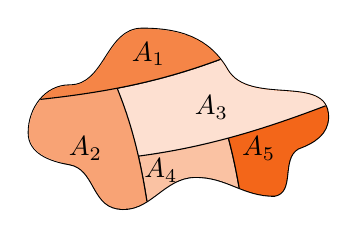
\begin{tikzpicture}[scale=0.4]
\path
  coordinate (aux0) at (0,1.5)
  coordinate (aux1) at (0,3.5)
  coordinate (aux2) at (10,3.5)
  coordinate (aux3) at (9,6)
  coordinate (aux4) at (4,0)
  coordinate (aux5) at (7,0)
  coordinate (aux6) at (2,6)
  coordinate (aux7) at (5,6)
  coordinate (esp1) at (0.2,2.5)
  coordinate (esp2) at (1.5,1.5)
  coordinate (esp3) at (3,0.1)
  coordinate (esp4) at (5.5,1.1)
  coordinate (esp5) at (8,0.5)
  coordinate (esp6) at (8.75,2)
  coordinate (esp7) at (9.7,3)
  coordinate (esp8) at (6.5,4.5)
  coordinate (esp9) at (3.8,5.8)
  coordinate (esp10) at (1.5,4)
  ;
\draw[line width=0.8pt]
  (esp1) to[out=-90,in=170]
  (esp2) to[out=-10,in=170]
  (esp3) to[out=-10,in=180]
  (esp4) to[out=0,in=180]
  (esp5) to[out=10,in=-150]
  (esp6) to[out=20,in=-90]
  (esp7) to[out=90,in=-60]
  (esp8) to[out=120,in=0]
  (esp9) to[out=180,in=0]
  (esp10) to[out=180,in=90]
  cycle;    
\clip
  (esp1) to[out=-90,in=170]
  (esp2) to[out=-10,in=170]
  (esp3) to[out=-10,in=180]
  (esp4) to[out=0,in=180]
  (esp5) to[out=10,in=-150]
  (esp6) to[out=20,in=-90]
  (esp7) to[out=90,in=-60]
  (esp8) to[out=120,in=0]
  (esp9) to[out=180,in=0]
  (esp10) to[out=180,in=90]
  cycle;    
\filldraw[fill=ocre!40]
  (aux4) to[bend right=10]
  (aux6) --
  (aux7) to[bend left=10]
  (aux5) -- cycle;
\filldraw[fill=ocre]
  (aux5) to[bend right=10]
  (aux7) --
  (10,6) --
  (10,0) -- cycle;
\filldraw[fill=ocre!20]
  (aux0) -- 
  (aux1) to[bend right=10]
  (aux3) --
  (10,6) -- 
  (aux2) to[bend left=10] cycle;
\filldraw[fill=ocre!60]
  (0,0) -- 
  (aux4) to[bend right=10]
  (aux6) --
  (0,6) -- 
  (0,0) -- cycle;
\filldraw[fill=ocre!80]
  (0,6) -- 
  (aux1) to[bend right=10]
  (aux3) --
  (0,6) -- cycle;
\node at (4,5) {$A_1$};  
\node at (2,2) {$A_2$};  
\node at (6,3.3) {$A_3$};  
\node at (4.4,1.3) {$A_4$};  
\node at (7.5,2) {$A_5$};  
\node at (7,5) {$\Omega$};  
\end{tikzpicture}
\end{center}
\end{minipage}

\end{definition}


\begin{proposition} Soit $n$ un entier naturel non nul et $A_1$, $A_2$, ..., $A_n$ des ensembles finis deux à deux disjoints.
\[ \Card(A_1 \cup A_2 \cup \ldots  \cup A_n)= \Card(A_1) + \Card(A_2)+\ldots + \Card(A_n)= \sum_{i=1}^n \Card(A_1)\]
\vspace{-0.5cm}\end{proposition}

Une approche possible du dénombrement est d'établir une disjonction de cas pour découper le problème que l'on étudie en d'autres problèmes plus petits que l'on sait dénombrer. Ceci rappelle naturellement la \textbf{formule des probabilités totales}.

\begin{example}Un tournoi de mathématiques est organisé entre 256 joueurs. A chaque manche du tournoi, les participants sont répartis en groupes de 4 candidats et chaque groupe se voit alors attribuer une épreuve à l'issue de laquelle un seul candidat parmi les 4 du groupe pourra se qualifier. A la fin de ce tournoi, il n'y a qu'un seul vainqueur. Combien d'épreuves auront lieu au total ?

\vskip150pt

\end{example}
Tout ce raisonnement peut vous sembler inutilement compliqué pour une situation aussi simpliste que celle-là, mais il faut parfois savoir préciser à outrance les objets et les ensembles que l'on manipule pour être certains que les outils mathématiques que nous utilisons sont les bons.

\begin{proposition}[Formule du crible]
Soit $A$ et $B$ des ensembles finis
\[ \Card(A \cup B) = \Card(A) + \Card(B) - \Card( A\cap B)\]\vspace{-0.5cm}\end{proposition}
\begin{minipage}{0.65\linewidth}
Si l'on compte le nombre d'éléments de $A$ et que l'on ajoute le nombre d'éléments de $B$, certains éléments ont alors été compté deux fois : ceux communs à $A$ et $B$ (c'est-à-dire les éléments de $A\cap B$).

En retirant le nombre d'éléments de cette intersection à notre compte, on obtient alors le nombre d'éléments de l'union.
\end{minipage}\hfill\begin{minipage}{0.3\linewidth}
\newcommand{\A}{(0,0) ++(135:2) circle (2)}
\newcommand{\B}{(0,0) ++(45:2) circle (2)}
\begin{tikzpicture}[scale=0.6]

\draw [thick,black] \A ; 
\draw [thick,black] \B ; 
 \fill[ocre!40, opacity=0.5] \A; \fill[blue!40, opacity=0.5] \B;
 \node at (-2,0) {$A$};
  \node at (2,0) {$B$};
  \node at (0,1) {$A\cap B$};
  
\end{tikzpicture}
\end{minipage}

Encore une fois, la liaison est à faire avec les probabilités et la formule $\mathbb{P}(A\cup B)=\mathbb{P}(A)+\mathbb{P}(B)-\mathbb{P}(A \cap B)$.

\begin{example}Pour accompagner leurs frites à la cantine, 150 élèves choisissent leur sauce entre ketchup et mayonnaise (éventuellement les deux). On suppose que tous les élèves ont pris au moins une sauce. Par ailleurs, 92 élèves ont pris du ketchup et 97 ont pris de la mayonnaise. Combien ont pris les deux sauces ?

\vskip50pt

\end{example}
\newpage
\subsection{Produit cartésien}

\begin{definition} Soit $A$ et $B$ deux ensembles.
 
 \begin{itemize}
 \item On appelle \textbf{produit cartésien} de $A$ et $B$, noté $A \times B$ ($A$ "croix" $B$), l'ensemble composé des couples $(a;b)$ avec $a \in A$ et $b \in B$. 
 \item Le produit cartésien $A\times A$ est également noté $A^2$.
\end{itemize}\end{definition}

\begin{example}On considère les ensembles $A=\{2;5;9\};$ et $B=\{3;5\}$.
\begin{itemize}
\item  Les éléments de $A \times B$ sont 
\item Les éléments de $B \times A$ sont 
\item Les éléments de $B^2$ sont 
\end{itemize}\end{example}

On remarque sur cet exemple que le produit cartésien n'est pas commutatif !

\begin{definition} La notion de \textbf{produit cartésien} s'étend naturellement à plus de deux ensembles. 
\begin{itemize}
 \item Soit $n$ un entier naturel supérieur ou égal à 2. le produit cartésien de $n$ ensembles $A_1$, $A_2$, ..., $A_n$ est l'ensemble des $n$-uplets $(a_1;a_2;\ldots;a_n)$ avec $a_1 \in A_1$, $a_2 \in A_2$, ... $ a_n \in A_n$.
 \item Le produit cartésien $A \times A \times ... \times A$ où $A$ apparaît $n$ fois est noté $A^n$. Ses éléments sont appelés les $n$-\textbf{uplets} de $A$.\end{itemize}
\end{definition}

\begin{example} On considère les ensembles $A=\{1;2;4\}$, $B=\{3;7;14\}$ et $C=\{1;3\}$.
\begin{itemize}
\item $(1;7;3) \in A \times B \times C$ puisque $1 \in A$, $7 \in B$ et $3 \in C$.
\item $(3;7;7;3;14) \in B^5$ puisque $3$, $7$ et 14 sont dans l'ensemble $B$.
\end{itemize}\end{example}

\begin{proposition} Soit $A$ et $B$ des ensembles finis. 
\begin{itemize}
\item $\Card (A \times B)=\Card(A) \times  \Card (B)$.
\item Plus généralement, soit $n$ un entier naturel, $A_1$, $A_2$, ..., $A_n$ des ensembles finis. \[\Card(A_1 \times A_2 \times \ldots \times A_n)=\Card(A_1) \times \Card(A_2) \times \ldots \times \Card(A_n).\]
\item En particulier, pour tout entier naturel $n$, on a $\Card(A^n)=[\Card(A)]^n$.
\end{itemize}\end{proposition}


\begin{example} On reprend les ensembles $A=\{1;2;4\}$, $B=\{3;7;14\}$ et $C=\{1;3\}$. On a
\begin{itemize}
\item $\Card(A \times B)= $
\item $\Card(A \times B \times C) = $
\item $\Card(A^4)=$
\item $\Card(C^{10})=$
\end{itemize}\end{example}

\newpage

\begin{proposition} Le produit cartésien est utilisé pour dénombrer des situations où l'ordre des symboles (chiffres, lettres, signes...) est important et où ces symboles peuvent être utilisés plusieurs fois.\end{proposition}

\begin{example} A l'entrée d'un bâtiment est installé un digicode. Pour composer le code, on utilise 4 chiffres compris entre 1 et 6 suivis de deux lettres parmi les lettres A, B, C et D. Un chiffre ou une lettre peuvent être utilisés plusieurs fois. Combien de codes sont possibles ?


\vskip40pt
\end{example}


\section{Arrangements et permutations}


\begin{definition}Soit $n$ un entier naturel non nul. On note $n!$ (\textbf{factorielle} de $n$) le produit de tous les entiers de 1 à $n$. Ainsi, $n!=n\times (n-1) \times \ldots \times 2 \times 1$.

Par ailleurs, on convient que $0!=1$.\end{definition}

Il est également possible de définir la factorielle par récurrence, en stipulant que $0!=1$ et que, pour tout entier naturel $n$, $(n+1)!=(n+1) \times n!$. Cette version de la factorielle a notamment été rencontrée par les élèves suivant la spécialité NSI lors de leur premier contact avec la récursivité.

\begin{example} $5!=\qquad\qquad\qquad\qquad\qquad\qquad\qquad\qquad \dfrac{8!}{6!}=$\end{example}

\begin{definition}Soit $A$ un ensemble fini de cardinal $n$ et $k$ un entier inférieur ou égal à $n$. 

Un $k$-\textbf{arrangement} de $A$ est un $k$-uplet d'éléments distincts de $A$.

Lorsque $k=n$, on parle de \textbf{permutation} de $A$.\end{definition}

\begin{example} On considère l'ensemble $A=\{1;3;4;5;7;10\}$. 
\begin{itemize}
\item $(7;10;3)$ est un 3-arrangement de $A$. 
\item $(10;5;4;1)$ est un 4-arrangement de $A$. 
\item En revanche, $(7;10;1;7)$ n'est pas un arrangement de $A$ car l'élément $7$ y apparaît deux fois. 
\item $(3;7;4;5;1;10)$ est par ailleurs une permutation de $A$ puisque tous les éléments de $A$ y apparaissent.
\end{itemize}
\vspace{-0.5cm}\end{example}

 
 \begin{proposition}Soit $A$ un ensemble fini de cardinal $n$ et $k$ un entier inférieur ou égal à $n$. 
 
 Le nombre de $k$-arrangements de $A$ vaut $\dfrac{n!}{(n-k)!}$.
 
 En particulier, le nombre de permutation de $A$ vaut $n!$.\end{proposition}
 
\begin{demonstration} Pour construire un $k$-uplet d'éléments distincts de $A$, on a
 \begin{itemize}
 \item $n$ choix pour le premier élément
 \item $n-1$ choix pour le deuxième
 \item ...
 \item $n-(k-1)$ pour le $k$-ième
 \end{itemize}
 Le nombre de $k$ arrangements de $A$ vaut donc $n \times (n-1) \times \ldots \times n-(k+1)$, ce que l'on peut réécrire en 
 \[ n \times (n-1) \times \ldots \times (n-(k-1)) \times \dfrac{(n-k) \times (n-k-1)\times \ldots \times 2 \times 1}{(n-k) \times (n-k-1)\times \ldots \times 2 \times 1}=n \times (n-1) \times \ldots \times (n-(k-1)) \times \dfrac{(n-k)!}{(n-k)!}\]
 d'où
 \[n \times (n-1) \times \ldots \times( n-(k-1)) \times \dfrac{(n-k) \times (n-k-1)\times \ldots \times 2 \times 1}{(n-k) \times (n-k-1)\times \ldots \times 2 \times 1}=\dfrac{n!}{(n-k)!}.\]\end{demonstration}
 
\begin{example} On considère l'ensemble $A=\{1;3;4;5;7;9;11\}$, de cardinal 7. 

Le nombre de $3$-arrangements de $A$ vaut \end{example}


 
\begin{proposition} Les arrangements sont utilisés pour dénombrer des situations où l'ordre des objets (chiffres, nombres, lettres, signes,...) est important mais où chaque objet ne peut être utilisé qu'une seule fois.\end{proposition}

\begin{example}Une cours hippique réunit 8 jockeys et leurs chevaux. Le "quarté dans l'ordre" est un pari qui consiste à deviner les quatre premiers chevaux arrivés dans l'ordre. Combien de paris différents est-il possible de réaliser ?

\vskip100pt

\end{example}
 

 \section{Combinaisons d'un ensemble fini}
 
 \begin{definition} Une \textbf{partie} ou \textbf{combinaison} d'un ensemble fini $A$ est un ensemble inclus dans $A$. L'ensemble des parties de $A$ est noté $\mathcal{P}(A)$.\end{definition}


\begin{example} Soit $A=\{1;2;3\}$. Les parties de $A$ sont $\varnothing$, $\{1\}$, $\{2\}$, $\{3\}$, $\{1;2\}$, $\{1;3\}$, $\{2;3\}$ et $\{1;2;3\}$. Elles sont au nombre de $8$

Attention à ne pas oublier l'ensemble vide $\varnothing$ et l'ensemble complet $A$ lui-même en établissant cette liste.\end{example} 
 
 \begin{proposition}
Soit $A$ un ensemble fini de cardinal $n$. Le nombre de parties de $A$ est $2^n$.\end{proposition}
 
\begin{demonstration} Nous allons montrer qu'il y a autant de parties de $A$ que de $n$-uplets de l'ensemble $\{0;1\}^n$. Puisque $\{0;1\}$ possède 2 éléments, le cardinal de $\{0;1\}^n$ vaut donc $2^n$.
 
 Pour cela, à chaque partie de $A$, on fait correspondre un élément de $\{0;1\}^n$ de telle sorte que deux parties différentes de $A$  sont associés à deux $n$-uplets différents de $\{0;1\}$. On dit qu'on réalise une bijection entre $\mathcal{P}(A)$ et $\{0;1\}^n$.
 
 L'idée : Pour chaque élément de $A$, on a deux choix pour construire une partie de $A$ : soit cet élément appartient à la partie que l'on construit, soit il ne lui appartient pas. 

\newpage 
 
 On a donc
 \begin{itemize}
 \item 2 choix pour le premier élément de $A$
 \item 2 choix pour le deuxième élément...
 \item ...
 \item 2 choix pour le $n$-ième élément de $A$.
 \end{itemize}
 Ainsi, le cardinal de $\mathcal{P}(A)$ vaut $2\times 2 \times \ldots \times 2 = 2^n$.
 
 
De manière formelle : Notons $a_1$, $a_2$ , ..., $a_n$ les éléments de $A$. 
  Soit $B$ une partie de $A$. On construit un $n$-uplet $(b_0;b_1;...;b_n)$ de $\{0;1\}$ comme suit : pour tout entier naturel $i$ entre 1 et $n$
  \begin{itemize}
  \item $b_i=1$ si $a_i \in B$
  \item $b_1=0$ sinon.
  \end{itemize}
Chaque partie de $A$ est ainsi associé de manière unique à un $n$-uplet de $\{0;1\}$ et réciproquement. Les cardinaux de $\mathcal{P}(A)$ et $\{0;1\}^n$ sont donc égaux.\end{demonstration}



\begin{definition} Soit $A$ un ensemble fini à $n$ éléments et $k$ un entier naturel $n$. 

Le nombre de combinaisons à $k$ éléments de $A$ est noté $\dbinom{n}{k}$ et se lit "$k$ parmi $n$". 

Les nombres $\dbinom{n}{k}$ sont appelés coefficients binomiaux\end{definition}

\begin{example}Soit $A=\{1:2:3:4:5\}$. 

Les parties à deux éléments de $A$ sont 

Il y en a $\qquad$ : ainsi, $\dbinom{5}{2}=$\end{example}

Attention, l'ordre n'a pas d'importance lorsque l'on parle de partie d'un ensemble : le sous-ensemble $\{1;2\}$ est le même que le sous-ensemble $\{2;1\}$.


\begin{proposition} Soit $n$ et $k$ deux entiers naturels.
\begin{itemize}
\item Si $k > n$, $\dbinom{n}{k}=0$ ;
\item Sinon, $\dbinom{n}{k} = \dfrac{n!}{k!(n-k)!}$.
\end{itemize}\end{proposition}

\begin{demonstration}On sait qu'il y a $\dfrac{n!}{(n-k)!}$ $k$-arrangements de $A$. 

Cependant, plusieurs $k$-arrangements utilisent les mêmes éléments de $A$ (par exemple, les couples (1;2) et (2;1) utilisent les nombres 1 et 2). 

Étant donnée une partie de $A$ à $k$ éléments, on peut construire $k!$ arrangements différents : on a $k$ choix pour le premier élément, $k-1$ pour le deuxième, etc.

Ainsi, le nombre de $k$-arrangements est $k!$ fois plus grand que la nombre de combinaisons à $k$ éléments. Ainsi, le nombre de combinaisons à $k$ éléments est égale au nombre de $k$-arrangements divisé par $k!$, soit $\dfrac{n!}{k!(n-k)!}$.\end{demonstration}

\newpage

\begin{example} Soit $A=\{1;2;3;4\}$. 

Le nombre de parties de $A$ à deux éléments vaut \\ 
\vskip5pt Ces parties sont\end{example}



\begin{proposition} Soit $n$ un entier naturel non nul. 

\begin{tabularx}{\linewidth}{X|X}
Pour tout entier naturel $k \leqslant n$, $\dbinom{n}{k}=\dbinom{n}{n-k}$. & $\dbinom{n}{0}=\dbinom{n}{n}=1$. \\
\hline
Si $n\geqslant 1$, $\dbinom{n}{1}=\dbinom{n}{n-1}=n$. & Si $n\geqslant 2$, $\dbinom{n}{2}=\dbinom{n}{n-2}=\dfrac{n(n-1)}{2}$.
\end{tabularx}

\end{proposition}

\begin{demonstration} (Avec la formule) :
\begin{itemize}
\item Pour tout entier naturel $k\leqslant n$, $\dbinom{n}{n-k}=$.
\vskip10pt
\item D'après le premier point, on a bien $\dbinom{n}{0}=\dbinom{n}{n-0}=\dbinom{n}{n}$. Or, $\dbinom{n}{0}=$
\vskip10pt
\item D'après le premier point,  $\dbinom{n}{1}=\dbinom{n}{n-1}$. Or, $\dbinom{n}{1}=$
\vskip10pt
\item D'après le premier point,  $\dbinom{n}{2}=\dbinom{n}{n-2}$.

 Or, $\dbinom{n}{2}=$
\end{itemize}\end{demonstration}






\begin{demonstration} (Démonstration combinatoire)

\begin{itemize}
\item Choisir $k$ objets parmi $n$ revient à exclure $n-k$ objets parmi ces $n$ objets. Ainsi, $\dbinom{n}{k}=\dbinom{n}{n-k}$.
\item Il n'existe qu'un seul ensemble à 0 élément, il s'agit de l'ensemble vide $\varnothing$. De la même manière, si $A$ est un ensemble à $n$ éléments, la seule partie de $A$ ayant $n$ éléments est l'ensemble $A$ lui-même.\\  Ainsi, $\dbinom{n}{0}=\dbinom{n}{n}=1$.
\item Si $A$ est un ensemble fini $\{a_1;a_2;\ldots ;a_n\}$ de cardinal supérieur ou égal à 1, les parties à 1 élément de $A$ sont simplement les singletons $\{ a_1\}$, $\{a_2\}$, ... , $\{a_n\}$. 

Ainsi, $\dbinom{n}{1}=\dbinom{n}{n-1}=n$.
\item Soit $A$ un ensemble de cardinal $n\geqslant 2$. Pour construire une partie à 2 éléments de $A$, on choisit un premier élément ($n$ choix possibles) puis un second ($n-1$ choix). En faisant ainsi, on peut construire $n(n-1)$ couples d'éléments de $A$. Or, l'ordre n'ayant pas d'importance, il est possible d'inverser l'ordre dans lequel on choisit les éléments de $A$. \\ Le nombre de combinaisons de $A$ à 2 éléments vaut donc $\dfrac{n(n-1)}{2}$
\end{itemize}\end{demonstration}

\begin{example} $\dbinom{100}{98}=$\end{example}



\begin{proposition}Les combinaisons sont utilisées pour dénombrer les situations où l'ordre des objets n'est pas important - lorsque l'on tire simultanément plusieurs personnes ou objets au hasard par exemple - et qu'un objet ne peut être utilisé qu'une seule fois.\end{proposition}

\begin{example} A la belote, on utilise un jeu de 32 cartes. Chaque carte est déterminé par sa couleur (Pique, Trèfle, Carreau, Coeur) et sa valeur (As, Roi, Dame, Valet, 10, 9, 8, 7). Pour le premier tour de distribution, chaque joueur reçoit 5 cartes, que l'on appelle une main. 

Quelle est la probabilité qu'une main contienne exactement deux as ?


\vskip200pt
\end{example}



\begin{proposition}Soit $n$ un entier naturel supérieur ou égal à 2 et $k$ un entier tel que $1\leqslant k\leqslant n-1$. On a alors
\[ \dbinom{n-1}{k-1}+\dbinom{n-1}{k} = \dbinom{n}{k}.\]
Cette relation s'appelle la relation de Pascal.\end{proposition}

\begin{demonstration}[Avec la formule] : On a
\[ \dbinom{n-1}{k-1}+\dbinom{n-1}{k}=\]

\vfill \end{demonstration}
\newpage

\begin{demonstration}[Combinatoire] : Soit $A$ un ensemble fini à $n$ éléments et $a\in A$. Soit $k$ un entier naturel compris entre 1 et $n-1$. 

\vskip350pt
\end{demonstration}


\begin{proposition}La relation de Pascal permet de construire récursivement les coefficients binomiaux. Ces coefficients peuvent être arrangés en triangle et forment ce que l'on appelle le triangle de Pascal.
\vskip5pt
\begin{minipage}{0.45\linewidth}
\begin{center}
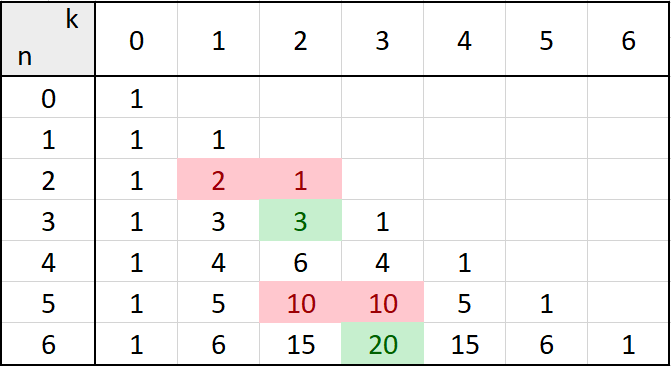
\includegraphics[scale=1.2]{pascal}
\end{center}
\end{minipage}\hfill\begin{minipage}{0.5\linewidth}
Dans ce triangle, on démarre avec un 1 en haut à gauche. Pour compléter chaque cellule, on ajoute alors le nombre au-dessus avec le nombre en haut à gauche. Les cases vides se voient assigner la valeur 0. On peut alors lire les coefficients binomiaux $\dbinom{n}{k}$ dans ce triangle.
\end{minipage}




\end{proposition}






\end{document}